
The integration of the components of the element stiffness matrix, the element mass matrix and
the consistent element load vector was analytically carried out in the previous chapters. In order to have in the development of complex finite elements an adequate tool for the integration of element quantities that are hardly integrable analytically, numerical integration is introduced
and examined for the truss example. By means of numerical integration, it is possible to integrate arbitrary functions in an approximate way. The essential advantages of numerical integration are summarized as follows:
\begin{itemize}
    \item Simplification of the integration
    \item Integration of analytically non-integrable functions
    \item Selective subintegration for elimination of defects from the element formulation
\end{itemize}
In opposition to these advantages there are actually limitations, too:
\begin{itemize}
    \item The generation of element matrices and vectors is numerically costly
     \item The element matrices and vectors are integrated inexactly 3

\end{itemize}

Within the framework of finite element methods, the so-called \textit{Gauss-Legendre Quadrature} has
established itself. The \textsc{Gauss-Legendre} Quadrature of a function $f(\xi 1)$ over the parameter
space $\xi_1 \in [−1, 1]$ is given by the sum
\begin{equation}
\label{eqn:2108}
     \int_{-1}^{1} f\left(\xi_{1}\right) d \xi_{1}=\sum_{i=1}^{n} \alpha^{i} f\left(\xi_{1}^{i}\right) 
\end{equation}
\begin{figure}[H]
    \centering
    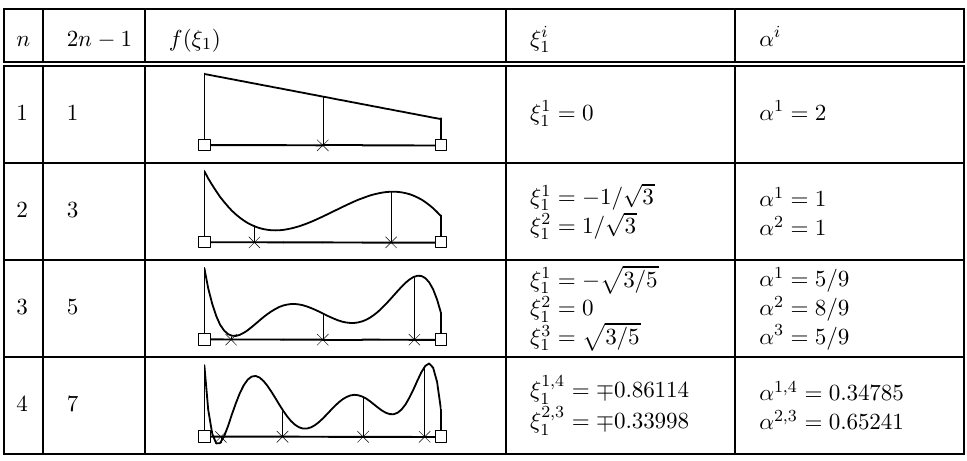
\includegraphics[scale=0.4]{Figures/Chapter2/quadrature.png}
    \caption{\textsc{Gauss} points $\xi_1^i$ and weight factors $\alpha^i$ of the \textsc{Gauss-Legendre} quadrature}
    \label{fig:222}
\end{figure}
In Eq. (\ref{eqn:2108}), $\alpha^i$ are the weight coefficients to the function values $f$ at the supports $\xi_1^i$ and n
is the number of integration points, or so-called \textit{Gauss points}. Polynomials of polynomial degree
\begin{equation}
    p\le 2n-1
\end{equation}
can be integrated exactly by \textsc{Gauss-Legendre} Quadrature, higher-order polynomials and other
functions can be integrated approximately. The linear, quadratic and cubic truss elements are
developed in this section by \textsc{Gauss-Legendre} integration with one and two supports. A summary of $\xi_1^i$ and $\alpha^i$ for $i = 1, 2, 3 $ is found in Figure \ref{fig:222}. For a representation of the fundamentals
of numerical integration, the way of obtaining of the weight factors $alpha^i$ and the \textsc{gauss} points $\xi_1^i$ , refer to the literature of numerical mathematics, e.g. \textsc{Deuflhard & Hohmann}

\textit{\underline{Example: Solve the equation:}}
\begin{equation*}
    x^3+x^2-5x=0
\end{equation*}
Code matlab and result for this problem :
\begin{lstlisting}
syms x;
F=x^3+x^2-5*x;
disp(int(F,[-1 1])); 
%% We take weight Gauss point from quadrature function
[Wgp,Qgp] = quadrature(5,'GAUSS',1); 
f=0;
%% Gauss Quadrature
for i=1 : size(Wgp,1)
    f=f+double(Wgp(i)*subs(F,x,Qgp(i)));
end
disp(f);
\end{lstlisting}

We have result for this example in Matlab : 
\begin{figure}[H]
    \centering
    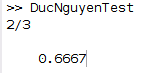
\includegraphics{Figures/Chapter2/resultQuadrature.png}
    \caption{Result for example Quadrature Problem}
    \label{fig:QDTP}
\end{figure}